\documentclass[conference]{IEEEtran}

\usepackage{amsmath}

\usepackage{graphicx}

\begin{document}

\title{General Drafts}



\maketitle


\begin{abstract}
A good abstract should answer the following few
questions. Question-1 what is the general topic of the article,
Question-2 what is the specific topic, Question-3 what is the
research problem, Question-4 what is the current status of the
problem and finally Question-5 what is the contribution(s) of the
article and/or work.
\end{abstract}

\section{INTRODUCTION}
This section is used to give little background and motivation
why to write this paper/article. More specifically a detail
answer of the questions from the abstract section



\section{METHODOLOGY}
To provide a framework/taxonomy to define the scope and
methodology, technical notations that you are going to use.

\section{MAIN BODY}
To list, describe and compare the leading work in the areas
using the uniform survey method/style that your have defined
in the above section. This section may contain some definition
like as follows:\\
\textit{Definition 1 (Composition anonymity):}For an individual i,
the composition anonymity offered by n independent k-
anonymized data sets is equal to the number of distinct
common sensitive values of the equivalence classes in which
the individual’s record resides.\\

\subsection{Part-1}
The numbers of sections and subsections are subject to your topic. This section may contain some equations like follows:

\begin{align}
	P(\hat{t}) &= P(\hat{q_1})\times P(\hat{q_{2}})\times ...\times P(\hat{q_{m}})\times P(s) \nonumber \\
&= (\prod_{i=1}^{m} P(\hat{q_{i}}))\times P(s)
\end{align}

\subsection{Part-2}
In end of each section and end of this paper, it is always a
good ideas to summarize your work by listing the technologies/
methods that you have discussed and compare them using
a table or figure.

\begin{table}[h]
\begin{center}
	\caption{COMMON NOTATION USED HERE}
	\label{notation}
	\begin{tabular}{ |c|c| } 
		\hline
		\textbf{Notation} & \textbf{Description}  \\ 
		\hline
		$\Omega$ & large population \\
		\hline 
		$D1, D_{1}, D_{2}$ & the original data sets\\
		\hline
		$ S^{d} $ & the set of \textit{d} different sensitive values\\
		\hline
		
	\end{tabular}
\end{center}
\end{table}

\vfill\null


\subsubsection{Table}
Draw a table as follows:
\begin{table}[h]
	\begin{center}
		\begin{tabular}{c|c|c}
			\hline
			Roll & Number & Position\\
			\hline
			1 & 2 & 3\\
			\hline
			4 & 5 & 6\\
			\hline
			7 & 8 & 9\\
			\hline
		\end{tabular}
	\end{center}
\end{table}

\subsection{Figure}
What a nice boat it is in Figure \ref{fig:boat}

\begin{figure}[h!]
	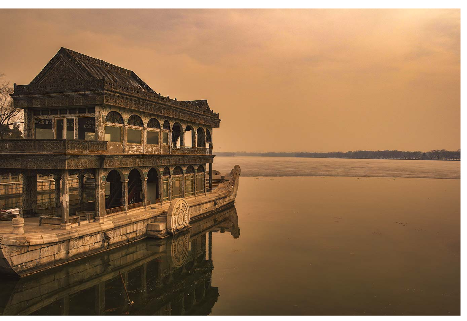
\includegraphics[width=\linewidth]{boat.jpg}
	\caption{A Boat}
	\label{fig:boat}
\end{figure}

\subsubsection{Table}
Draw a table as follows:
\begin{table}[h]
	\begin{center}
		\begin{tabular}{|c|c|c|c|}
			
			x & Method-1 & Method-2 & Method-3\\
			\hline
			5 & 101 & 98 & 55\\
			\hline
			10 & 98 & 105 & 60\\
			\hline
			15 & 96 & 120 & 70\\
			\hline
			20 & 110 & 130 & 100\\
			\hline
		\end{tabular}
	\end{center}
\end{table}


\begin{figure}[h!]
	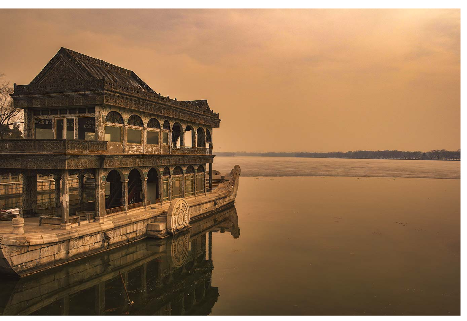
\includegraphics[width=\linewidth]{boat.jpg}
	\caption{A graph}
	\label{fig:boat}
\end{figure}



\section{REFERENCE TEST}
Referencing is one of the important parts of article writing. Let’s list some reference articles. This is \cite{Blum2005} a good conference paper. But, I like to read journal like \cite{Samarati:2001:PRI:627337.628183}. It is not a bad idea to read technical report like \cite{Li2011}.

\section{CONCLUSION}
Again summarize you work to show that you have successfully
achieved your objectives.

\bibliography{sarowar_ab} 
\bibliographystyle{ieeetr}
\end{document}